\begin{figure}[t!]
    \centering
    \vspace{-1ex}
    \begin{tikzpicture}
            \node[inner sep=0pt] (pic) at (0,0){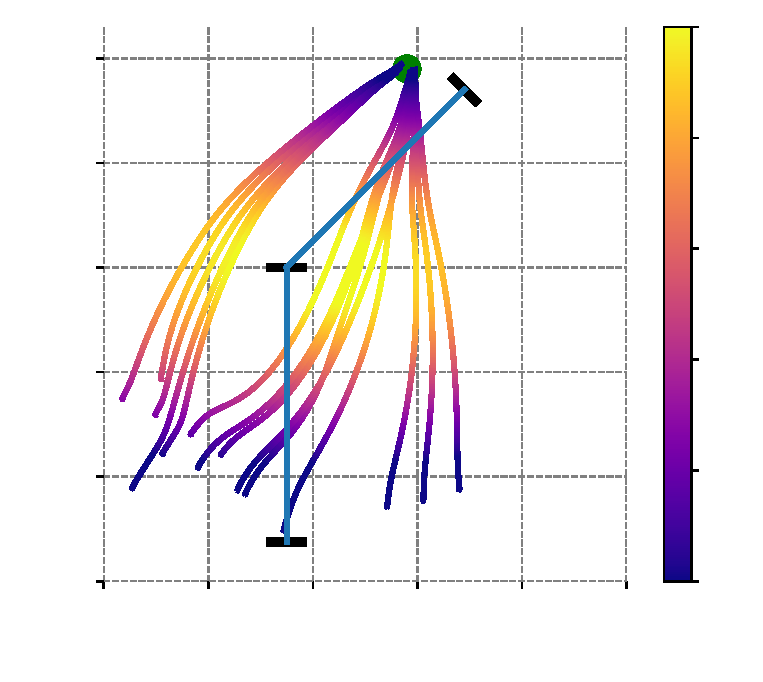
\includegraphics[width=1.0\columnwidth]{figures/fig_clean.pdf}};
            % x coodinate
            \node[inner sep=0pt] at (-3.15, -3.1){0};
            \node[inner sep=0pt] at (-1.96, -3.1){2};
            \node[inner sep=0pt] at (-1.96+1.19, -3.1){4};
            \node[inner sep=0pt] at (-1.96+1.19*2, -3.1){6};
            \node[inner sep=0pt] at (-1.96+1.19*3, -3.1){8};
            \node[inner sep=0pt] at (-1.96+1.19*4, -3.1){10};

            \node[inner sep=0pt] at (-1.96+1.19*1.5, -3.5){$x$ [m]};


            % y coordinate
            \node[inner sep=0pt] at (-3.5, -2.75){0};
            \node[inner sep=0pt] at (-3.5, -2.75 + 1.19){2};
            \node[inner sep=0pt] at (-3.5, -2.75 + 1.19*2){4};
            \node[inner sep=0pt] at (-3.5, -2.75 + 1.19*3){6};
            \node[inner sep=0pt] at (-3.5, -2.75 + 1.19*4){8};
            \node[inner sep=0pt] at (-3.5, -2.75 + 1.19*5){10};
            \node[inner sep=0pt, rotate=90] at (-3.9, -2.75 + 1.19*2.5){$y$ [m]};

            % colorbar
            \node[inner sep=0pt] at (4, -2.7) {0.0};
            \node[inner sep=0pt] at (4, -2.7+1.25) {0.2};
            \node[inner sep=0pt] at (4, -2.7+1.25*2) {0.4};
            \node[inner sep=0pt] at (4, -2.7+1.25*3) {0.6};
            \node[inner sep=0pt] at (4, -2.7+1.25*4) {0.8};
            \node[inner sep=0pt] at (4, -2.7+1.25*5) {1.0};

            %ABC
            \node[inner sep=0pt] at (-0.5, -2.3) {\large A};
            \node[inner sep=0pt] at (-1.45, 0.85) {\large B};
            \node[inner sep=0pt] at (1.4, 2.9) {\large C};

            %Goal
            \node[inner sep=0pt] at (-0.2, 3.5) {Goal};


    \end{tikzpicture}
    \caption{Visualization of the flown trajectories color-coded according to the values of $\alpha$, c.f. Sec.~\ref{sec:perception_aware_mpc}.
    Our MPC is able to find collision-free trajectories starting from non-collision-free reference trajectories.}
    \label{fig:sim}
\end{figure}